%!TEX root = ../main.tex
\chapter{Implementation}\label{chapter:implementation}
\section{Study of current Database}
Our main resource for the research was direct access the millions of Malware samples from Anubis collected over the years. Not only was this resource our main strength but it was also a challenge to effectively and efficiently analyze those data for our research works.\\
We started with studying the Anubis system and current database. We primarily dealt with two database of Anubis backend, the \textbf{db\_report} and \textbf{web\_analysis}.
The web analysis was the first entry of any sample malware submitted for analysis. It consisted of tables such as result, file, file\_task. Each sample was given a unique file\_id along with md5 and sha hashes.
A new file\_task \emph{id} was created  and the analysis of the sample would be done for different behavioral activities related to resources such as File, Registry, Mutex activities.
These activities were saved in db\_report database table. The resource activities of the malware in \textbf{db\_report} database was associated with the \textbf{web\_analysis} database by the constraint key \textit{result\_id} of \emph{result} table in web\_analysis database.
\begin{lstlisting}[language=sql,caption={sql showing database structure to get file created activities of a malware},label={lst:resultidsql}]
SELECT result_id FROM web_analysis.task join web_analysis.file_task using (task_id) join web_analysis.file using (file_id) WHERE task_id=result_id;
SELECT name from db_report.file_created join db_report.file_name using (file_name_id) where result_id ='12345';
\end{lstlisting}
We looked upon 3 resource type for the beginning. The resources type were \textit{File, Registry, Mutex}. For each resource type we took into account their \textit{create, read, delete} activities. The total number of malware sample that we had in our test database was \textbf{\gettotalmalwarei{}}.\\
Our first step was to create a reverse index from the database so that we could get the list of malware that is associated with the resource activities. We started with writing a python script to do the task and save it in the file.
However we found the first hurdle of our project. Since the number of malware were too large trying to save all their activities in data structure would cause our machine to run out of memory and hence crash the system. To solve this we took the approach of map reduce.\\
We ran our script in batch 50K malware at a time and saved the reverse index of activity to the file with numbering. Around 420 files were created for each resource type. The result files were in the format where resource name and list of result ids were separated by commas (,) as delimiter.
This was time consuming operation and it took almost 5 days for the script to finish. After the reverse index was generated in multiple numbered output, we sorted the file on resource name, alphabetically, and then joined the different parts with respect to the resource activity as key, and merged it into one single file.
Since, this was a merge sort, we considered two sorted files at a time until single file was left, the reduce part was pretty fast (Big O $O( n * \log(n))$).

\begin{lstlisting}[numbers=none]
  LANG=en_EN sort -t, -k 1,1 $file_name
  LANG=en_EN join -t , -a1 -a2 $file_name
\end{lstlisting}
The snippet of resultant output:
\begin{lstlisting}[numbers=none]
Application Data,87623151,87079727,87034095
AutoHotkey,87623151,87079727,87034095
AutoScriptWriter,87623151,87079727,87034095
B:\mbr.exe,121858971
BIN,177509111,103858187
Base Images,189524063,184501719,87504631,86763863
Buttons,111448211
C:/DOCUME~1/ADMINI~1/LOCALS~1/Temp/Adobe Reader 8,178046895,174206059,183601891,89650247
C:/DOCUME~1/ADMINI~1/LOCALS~1/Temp/_MEI1192/,161552035,116241803
\end{lstlisting}

\section{Packer \& Unpacker}
\label{sec:packerunpacker}
In order to run the pair of malware together in side the Anubis environment we made a Win32 console application, named Unpacker, as Anubis VM was Windows XP based. The notion behind this Unpacker binary is like a dropper, where a single binary will unpack itself to create two binary and run each of them.
We wrote a packer script that would add the candidate binary pair at the end of Unpacker binary and then further append the time delay and file size of each candidate binary as meta information.
The unpacker binary when executed would read itself to fetch the meta information and then the candidate binary bytes.\\
\begin{figure}[htbp]
  \centering
  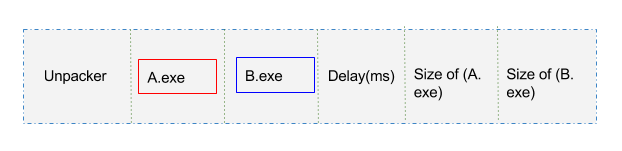
\includegraphics[scale=0.5]{figures/unpacker.png}
\caption{[Packer structure] Structure of the Packer binary that would create the candidate pair and run them with delay.}
\label{fig:unpacker}
\end{figure}
We used a struct of 3 integer size to read and hold the meta information. The size of last three \textit{unsigned int} byte had the binary pair sizes information and delay, know as meta information. The offset would be deduction of $3 * \textit{size of uint}$ from the total size of itself. When the file size of packed binary was known, we used \texttt{fseek\(\)} function appropriately to start reading form the correct position until the exact size of binary were read. Then these bytes were saved to the new file pointer. Once the binary pairs were extracted by the unpacker new binary files were created in the Anubis environment and those were executed one after another with the delay of time as given in meta information. We used \texttt{windows.h} standard libraries \emph{CreateProcess} and \emph{Sleep} function for the purpose.\\

\begin{lstlisting}[language=c,caption={snippet of unpacker.c file}, label={lst:unpacker.c}]
  /* stuct for storing meta information */
  typedef struct {
    unsigned int delay;
    unsigned int fsize1;
    unsigned int fsize2;
  }meta_info;

  /* reading the meta information and first binary */
  rfp = fopen(argv[0], "rb");
  wfp1 = fopen(fileName1, "wb");

  fseek(rfp,0,SEEK_END);
  size = ftell(rfp);
  offset = size - sizeof(meta_info);
  fseek(rfp, offset, SEEK_SET);
  fread(&info, 1, sizeof(info), rfp);

  /* calculate the unpackersize from the offset and files size. */
  unpackersize = offset - (info.fsize1 + info.fsize2);

  /* rewind back and to the point of the start of file1 */
  fseek(rfp,0,SEEK_SET);
  fseek(rfp, unpackersize, SEEK_SET);

  nread_sofar = 0;
  while (nread_sofar < info.fsize1) {
      nread = fread(buf, 1, min(info.fsize1 - nread_sofar, sizeof(buf)), rfp);
      nread_sofar += nread;
      fwrite(buf, 1, nread, wfp1);
  }
  fclose(wfp1);
 \end{lstlisting}
\section{Initial Experiment}
\label{sec:Initial Experiment}
From the reverse index of the resource activities of the Malware, we created a mapping between the created activities against the deleted or read activities.
We created a list of malware based on the common resource name as the key, where a list of malware created the resource and another list of malware delete/read the same resource.
We started looking for one to one interaction of malware to a single resource. Any resource type that was created by exactly single malware and deleted by exactly another single malware.
We looked for a set $(a, b)$, where malware `a' creates the resource \emph{r}, and malware `b' deletes the same resource, \emph{r}, and no other malware has create or delete activities on that resource \emph{r}.\\
After finding such pairs, when we ran those malware pairs in the Anubis system using our unpacker, we found lots of dropper malware causing this interaction. Binary `a' was a dropper that would create many binaries including the binary `b', and binary `b' actually read itself upon execution, which was recorded as read activity by Anubis.
After running many other candidate pairs with different interaction and analyzing the results manually, not only were we able to understand the Anubis report in depth but also found an error on our approach.\\
Our notion behind checking the malware interaction was finding candidate pairs such that one malware `a' creates some resource, `r', and another malware `b' tries to access or delete the same resource,`r'.
But since Anubis ran each submitted binary in an isolated environment, there was no way that a malware `b' would find the resource that was supposed to be created by malware `a'.
We should have been looking for failed attempt activities, where a malware unsuccessfully tried to access or delete a resource created by another malware, but the current database that we had did not had record of such failed attempt.
This lead for us to look for the alternatives were we could find log of such failed attempt activities.\\
\section{Behavioral Profile}
\label{sec:behvairoalprofile}
Previously,~\citeauthor{bayer} used Anubis system for the dynamic analysis of malware to gets it execution traces~\cite[]{bayer}.
They created a behavioral profile based on the execution traces of programs irrespective of order execution. It consisted a list of different operations operated on the different OS objects during the execution of binary.
We had these behavioral profiles saved as python pickle file in our system and we used this to recreate new database according to our need.
\begin{lstlisting}[language=TeX,caption={Behvaioral Profile sample}, label={lst:bpsample}]
  op|file|'C:\\Program Files\\Common Files\\sumbh.exe'
   create:1
   open:1
   query:1
   query_file:1
   query_information:1
   write:1

  op|registry|'HKLM\\SOFTWARE\\CLASSES\\CLSID\\{00021401-0000-0000-C000-000000000046}\\INPROCSERVER32'
   open:1
   query:1
   query_value(''):1
   query_value('InprocServer32'):0
   query_value('ThreadingModel'):1

  op|section|'BaseNamedObjects\\MSCTF.MarshalInterface.FileMap.ELE.B.FLKMG'
   create:1
   map:1
   mem_read:1
   mem_write:1
\end{lstlisting}
\section{Creation of Database}
\label{sec:Creation of Database}
Recreating the database was one of the bottleneck in our project and consumed much time.
The profile files were needed to be accessed via network file system, walking through list of directories and file to find the profile pickle of malware.
Not all of the profile pickle were found. We found \emph{\gettotalmalwareii{}} out of \emph{\gettotalmalwarei{}} malware.\\
We mapped the Windows Native and Windows Api call into three category modified, accessed, and delete.
We took only 8 of the resource type into account while parsing the profile files; those were File, Registry, Sync, Section, Process, Mutex, Job, and Driver
We went through the most common used API calls and then mapped them into the broad three categories as described earlier.

\begin{lstlisting}[language=ruby,caption={Mapping of WinodowsNT and Windows API call},label={lbl:ntapi}]
MODIFY_LIST = {
        file:      ["create_named_pipe", "create_mailslot", "create", "rename", "lock", "set_information", "write", "unlock", "flush_buffer", "suspend", "map", "resume"],
        registry:  ["create", "restore_key", "save_key", "map", "set_value", "set_information", "compress_key", "lock", "resume", "suspend", "mem_write"],
        process:   ["create", "set_information", "suspend", "resume", "unmap", "map"],
        job:       ["assign", "set_information"],
        driver:    ["unload"],
        section:   ["create", "map", "unmap", "mem_write", "extend", "suspend", "resume", "set_information", "release"],
        sync:      ["create", "release", "map", "set_information", "mem_write"],
        service:   ["create", "start", "control"]
        }

ACCESS_LIST = {
        file:      ["query_file", "query", "open", "query_directory", "query_information", "read", "monitor_dir", "control", "device_control", "fs_control", "query_value"],
        registry:  ["enumerate", "enumerate_value", "flush", "monitor_key", "open", "query", "query_value", "mem_read"],
        process:   ["open", "query"],
        job:       ["open", "query"],
        driver:    ["load"],
        section:   ["open", "query", "mem_read", "read", "query_file", "query_system"],
        sync:      ["open", "query"],
        service:   ["open"]
        }

DELETE_LIST = {
        file:      ["delete", "open_truncate"],
        registry:  ["delete", "delete_value"],
        process:   ["delete"],
        job:       ["delete"],
        driver:    ["delete"],
        section:   ["delete"],
        sync:      ["delete"],
        service:   ["delete"]
        }

\end{lstlisting}
We used MySql for the database and followed the previous table structure so that we could reuse our previous program on the newly created database.
The final database size was 1.2 Terrabytes. The basic CRUD operations were expensive and we hit the integer overflow for registry access activities table. We had to spent much time then expected on database tuning to make the program run faster to complete in reasonable time.
Most part of the execution time was taken to read the profile gzip pickle and then normal sql queries. This was for 17 million malware pickle profiles and their resource activities as defined above.
%TODO: put profile.png
After the creation of new database, we made a reverse index from the new refined data for the resource\_name and to malware ids modifying, accessing, and deleting the resource.
We again made the resource mapping taking into account those activity that had successful creation with those activities with failed access and another mapping between successful creation and delete activity.
We made this mapping for every resource types. So we had mapping between successful file creation and failed file deletion and mapping between successful file creation and failed file access.
Same was done for resource types registry, sync, section, mutex, job, and driver. The resource name was always the common key for the mapping between the malware.
We made a mapping like before and started to run the candidate pairs to test the behavioral interaction between the pairs. But, since the number of pairs were too many we hit the \emph{n-comination} problem.
A single resource \texttt{`r'} would have been created by more than thousands of malware and also same resource \texttt{`r'} would have been tried to access or delete with a failed attempt by another thousands of malware. If we made a pair out of every malware as possible candidate it would be too many candidates for us to run and analyze result.
We looked into clustering of the malware behavior to address this problem so that we could cluster malware on different topic and only choose one sample from the list of topic.
\section{Clustering}
\label{sec:Clustering}
We researched on many types of clustering algorithm that we could use to cluster our malware. Our idea of clustering was based on malware resource activities.
We had all the resource activities such as modification, access and deletion related to different resource types as discussed above.
We represented each resource type and activities as numeric value. And each resource name woul be represented by it's unique resource name id on our database system.
\begin{lstlisting}[language=python,caption={Numeric codes given to resource and operation},label={lbl:numericode}]
  RESOURCE_CODE    = {"file" : "1", "registry" : "2", "section" : "3", "service" : "4", "driver" : "5", "sync" : "6", "process" : "7", "job" : "8"}
  OPERATION_CODE   = {"access" : "1", "delete" : "2", "modify" : "3"}
\end{lstlisting}
So a file delete activity of filename, \textit{`c:\textbackslash\textbackslash{}gbot.exe'}, with file\_name\_id, ``4986'' in our database, by some malware ``A'', would be represented as single word ``1\_3\_4986''. Each such resource activities related to one single malware would be a bag of words representing  a single document representing that particular malware.\\
After days of running the script we could gather all the resource activity of {\gettotalmalwareii} malware. This was about 81 Gigabytes of data.
We used python module Gensim~\cite[Gensim]{gensim}  for the topic clustering and used the LDA model as described in Methodology section. We filtered our corpora by disacarding any resource activity that occurred in less than 1000 or more than 1 million for clustering.
This was based on heuristic after studying the cdf graph of activities to number of malware.
%TODO: add cdf of reverse index

The number of topic was chosen to be 1000, however our malware samples were distributed among only 752 unique topic.
\begin{lstlisting}[float,floatplacement=H,language=python,caption={Script to run Gensim LDA},label={lbl:lda.py}]
from gensim import corpora, models
import sys
document_name = sys.argv[1]
# read the file with malware activities and create dictionary
dictionary = corpora.Dictionary(line.split() for line in open(document_name))
# filter the dictionary for extreme
dictionary.filter_extremes(1000,0.6)
# create a iterator corpus as the file is large 80GB
class MyCorpus(object):
    def __iter__(self):
        for line in open(document_name):
            yield dictionary.doc2bow(line.split())

corpus = MyCorpus()
lda = models.ldamulticore.LdaMulticore(corpus=corpus,id2word=dictionary,num_topics=1000)
\end{lstlisting}
We calculated the distance between different clusters. We had quite a good results with small distance between the documents\(malware\) belonging to same cluster, intra topic distance, and larger distance between documents of different cluster, inter topic topic distance.
% \section{Weeding}
% \label{sec:Weeding}
\\
For the next Clustering run we wanted to decrease the number of malware\(documents\).
We did not had any resource activity mapping for resource type Mutex, Job, and Driver. Hence, we looked upon the remaining five resource type from our original resource types considered.\\
To do this we tried the manual approach. We sorted the reverse index of resource to malware with respect to the number of malware associated with the resource.
Once we had it sorted in descending order, we got most commonly modified/accessed/created resource at the top of the list, and went through all the mapping line by line until we found some interesting resource name.
Once we found that, we made a threshold to that resource name, and excluded any resource to malware mapping before that as it was not of substantial importance.\\
For instance, Resource with name such as \emph{Dr.\ Watson.exe} and \emph{Sample.exe} were the one with highest count of malware associated with it. The former one is created whenever the program crashes and the later one is the name that anubis uses to run the sample binary.
We looked for such benign resource names and weeded out for all the resource activities related to resource type file, registry, section, sync, and process. We were able to lower the total number of malware from {\gettotalmalwareii{}} to {\gettotalmalwareiii{}}.\\
We created the bag of words again for those {\gettotalmalwareiii{}} malware, and started the document clustering LDA algorithm. This time we had even better results with respect to inter distance and intra distance of the clusters.\\
The malware were clustered into 662 clusters. The largest cluster size was {\getlargestclustersize{}} and the lowest was {\getlowestclustersize{}}
The histogram and cumulative distributive graph showing the sizes of cluster can be seen in~\ref{fig:histclustersize},~\ref{fig:cdfclusterlen}, and~\ref{fig:ecdfclustersize}.\\
\begin{figure}
\begin{center}
  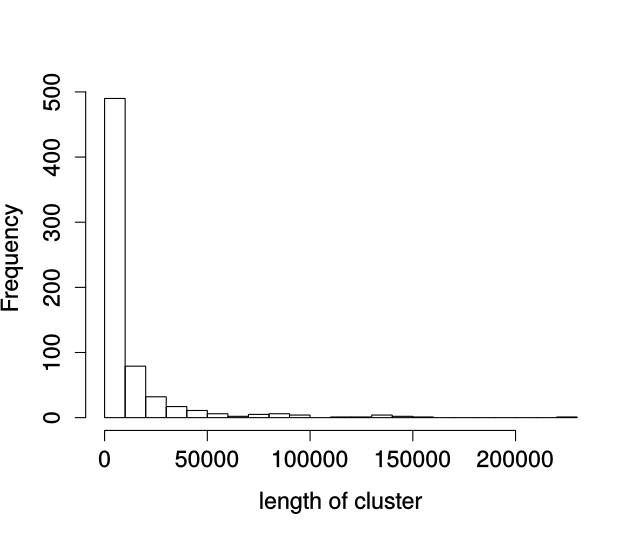
\includegraphics[scale=0.3]{figures/histclustersize.png}
\end{center}
\caption{Histogram showing the distribution of Cluster size}
\label{fig:histclustersize}
\end{figure}
\begin{figure}
\begin{center}
  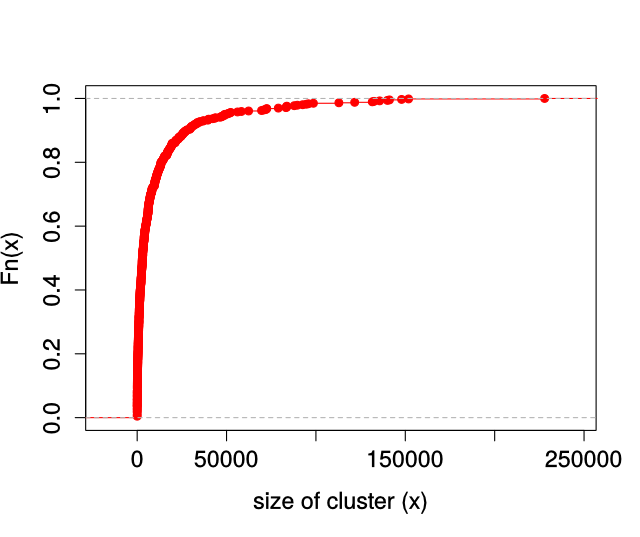
\includegraphics[scale=0.3]{figures/ecdfclustersize.png}
\end{center}
\caption{Graph showing cdf between size of cluster and topic fraction}
\label{fig:ecdfclustersize}
\end{figure}
\begin{figure}
\begin{center}
  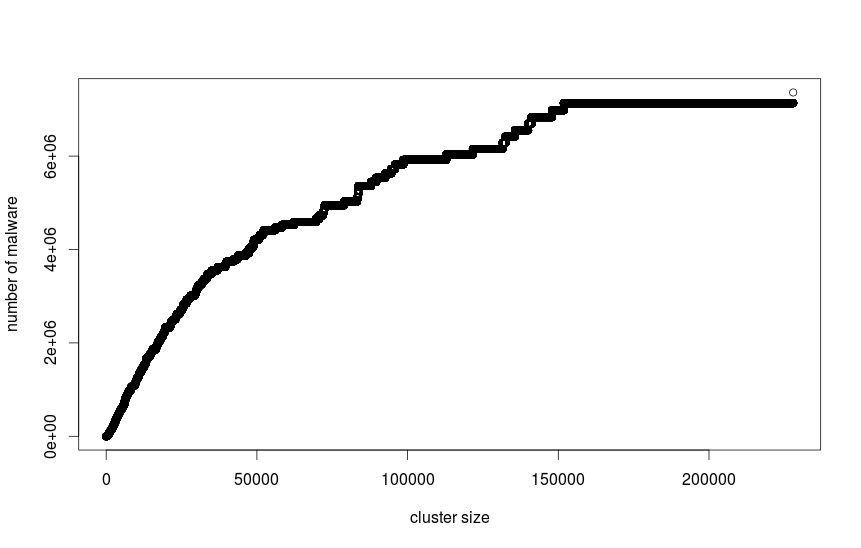
\includegraphics[scale=0.3]{figures/cdfclusterlen2.png}
\end{center}
\caption{Graph showing cdf between size of cluster and total number of malware}
\label{fig:cdfclusterlen}
\end{figure}
From the above graph we can see that distribution of cluster size was mostly below 50,000.
$90\%$ of the cluster topic, about \emph{629}, falls under the cluster size of less than 50,000, where as about \emph{4 million} malware, which is the $65\%$ of total malware, are in the clsuter size of less than 50K.\\
To see the quality of our clustering we present the following graph showing the graph of inter-cluster and intra-cluster distance in Figure~\ref{fig:interclustcommon} and Figure~\ref{fig:intraclustcommon}
In case of intra-distance, for each topic family, we sampled at maximum 1000 malware, if the topic had that many number of malware. We calculated the average number of resource activities\textit{(words)} present among those sampled mawlare\textit{(document)}
We then calculated the average common resources between the combinations of sample. We could see that the average common words between the intra malware sample were quite good with intra-distance of at least \emph{500} covering $80\%$ of family topics.
For the inter-distance calculation, we took a random combination pair of topic \emph{`x'} with other topics, and randomly sampled 1000 malware sample, if present, from those topic pair.
We calculated the average common words between those the sampled malware for each pair to find the inter distance between the malware of different family topics.
We found out the inter-distance of only 10 was covering almost $90\%$ of family topic.
\begin{figure}
\begin{center}
  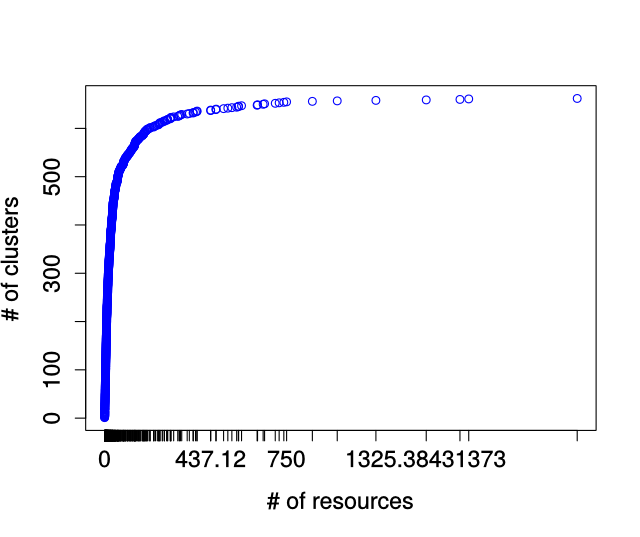
\includegraphics[scale=0.7]{figures/intra_clustered_common.png}
\end{center}
\captionsetup{font=small}
\caption{ Graph showing cdf distribution of common resource between same family topic}
\label{fig:intraclustcommon}
\end{figure}
\begin{figure}
\begin{center}
  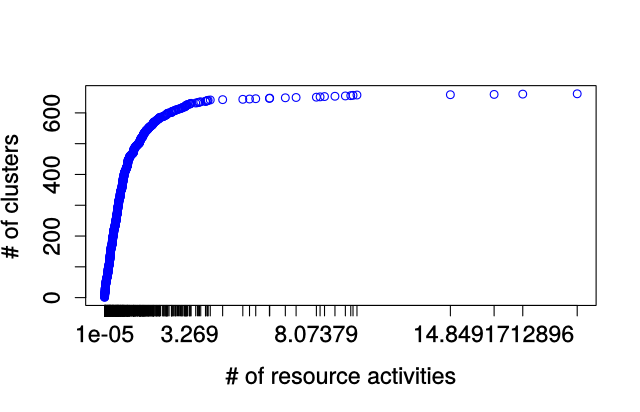
\includegraphics[scale=0.7]{figures/inter_clustered_common.png}
\end{center}
\captionsetup{font=small}
\caption{Graph showing cdf distribution of common resource between different family topic}
\label{fig:interclustcommon}
\end{figure}

\section{Finding out the candidate pairs}
\label{sec:Finding out the candidate pairs}
After the clustering of the malware was done, we used the result and the our mapping of resource to malware to find the candidate pairs for experiment.
In order to find the optimal set of candidate we interpreted the interaction of malware and resource with respect to cluster into Flow Network.
\subsection{Max Flow apporach}
\label{sub:Max Flow apporach}
We wanted to find the optimal pair of malware such that we have all the interesting mapped resource covered along with the cluster associated with it.
We represented the mapping between the resource, malware, and cluster as a flow network, and run the max flow algorithm as shown in Figure~\ref{fig:maxflow}, to yield the optimal solution.\\
The network is made of 4 layers, other than sink and source. Layer one is reading malware, the samples that tried to access or delete interesting resources but failed.
Layer two is combinations of clusters, \emph{ic=input cluster} that the malware with failed access or delete attempt belongs to, and the interesting resources that they tried to operate on.
Layer three is the combinations of clusters,\emph{oc=output cluster} that the malware with successful modification operation belongs to, and the interesting resources that they modified.
Layer four is the malware that successfully created the resource.\\
The flow rules were:
\begin{itemize}
  \item All malware from layer one is connected from source and also connected to the input cluster and resource combination it belongs to.
  \item All input cluster resource combination in layer two is connected to all output cluster resource combination in layer 3 that has a matching resource.
  \item All output cluster resource in layer 3 is connected to the corresponding malware in layer 4.
  \item Each malware in layer 4 is connected to the sink (T).
\end{itemize}
The capacities were:
\begin{itemize}
  \item All connections have capacity of infinite except connections from layer 2 to layer 3.
  \item All connections from layer 2 to layer 3 have a capacity of one.
  \item The maximum flow in this network is corresponding to an optimum match up.
\end{itemize}
Combinations and nodes that do not have a path from source to sink were not be put in the graph.\\
\begin{figure}[h]
  \centering
  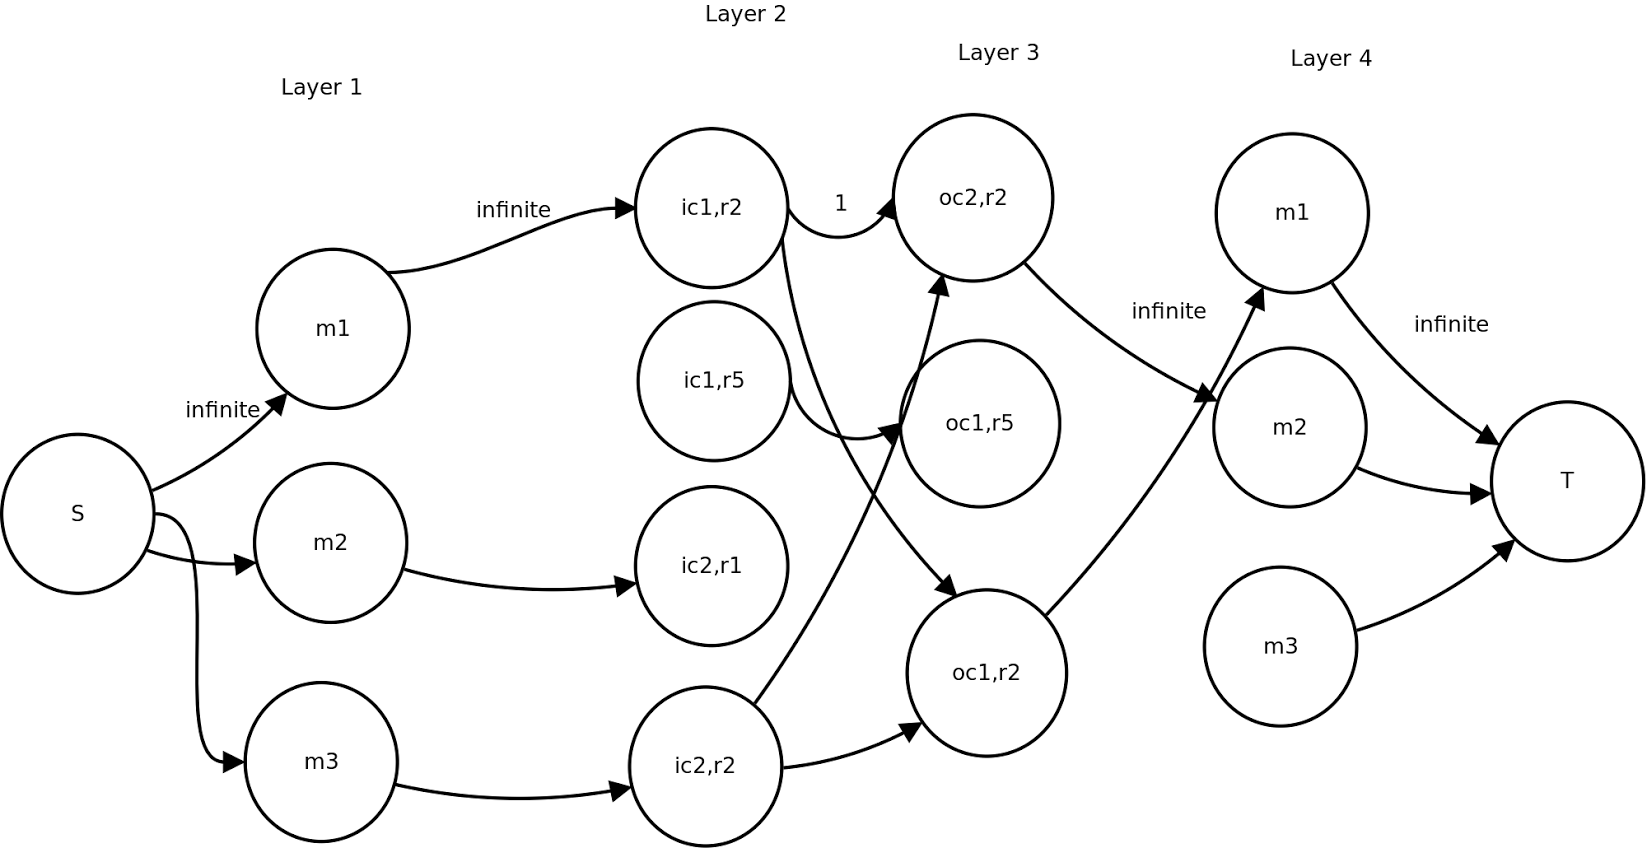
\includegraphics[scale=0.23]{figures/maxflow.png}
  \caption[Max Flow]{Graph representing the max flow implementation}\label{fig:maxflow}
\end{figure}
The thing wrong with this approach was the number of candidate pair to test were too many.
We wanted to decrease this number in such a way that there were no repetition of malware pair.
In order to achieve that, we tried Heuristic approach as described next.
\subsection{Heuristics Approach}
\label{sub:Heuristics Approach}
% We see in the first approach, we are not covering all resource interactions that were meticulously carved from millions of data points. 
The problem was to find the ``minimal set'' of md5 pairs that covers all unique family pairs (dictated by the set of all candidate pairs) and it also covers all resources that help build the candidate pairs, i.e., for each resource \emph{r} from resources \emph{R}, at least one md5\_pair from the final set should correspond the resource \emph{r}.
The relations has been represented in the graph below, where, \emph{I} is a set of input clusters from set \emph{`A'} and \emph{`O'} is the output clusters from set \emph{B}. Set \emph{A,B} and \emph{R} has usual meanings as described in the\textit{~\nameref{chapter:methedology} Section}.
\begin{figure}[htbp]
  \centering
  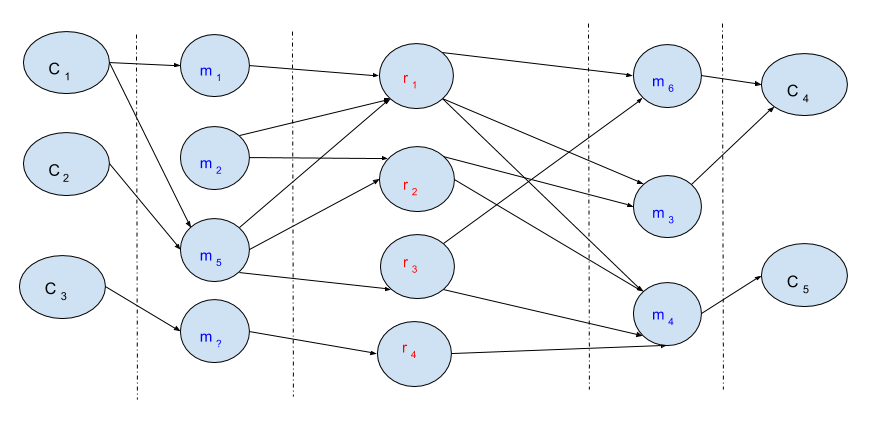
\includegraphics[scale=0.45]{figures/dhkherusitcs.png}
  \caption[]{Graph showing the interconnection between Cluster topics, Malware, and Resources.}\label{fig:dhkheuristics}
\end{figure}
\\
In the Figure~\ref{fig:dhkheuristics},  m1,m2, m5 samples create resource r1, which is accessed (failed attempt) by m6, m3, and m4.\ m1 and m2 maps to cluster c1. Malware m6 and m3 maps to cluster c4 \dots.
The problem is to find the minimal number of paths from each element \emph{c\_x} of set \emph{`I'} to all reachable elements in \emph{`O'} (reachable from \emph{c\_x}), such that all reachable elements \emph{`r'} in \emph{`R'} (reachable from \emph{c\_x}) are traversed. From such minimal set, we generated the candidate pairs by taking members of \emph{A} and \emph{B} from the path.
% This should work as we hard clusters (sample only falls into one cluster).
We created the following data structure as shown in~\ref{lst:dbdict}.
The data is a dictionary. All candidate cluster pairs are keys and the value is a dictionary whose keys are md5 pairs (all md5 pairs) and values are the list of corresponding resource ids.
\begin{lstlisting}[language=python,floatplacement=H,caption={Database Structure},label={lst:dbdict}]
db = { (c_i, c_o) :
    { (m_a, m_b) : [ r1, r2 ,...],
        ...,
     }
}
\end{lstlisting}
The reduced candidate set was computed as shown in below algorithm~\ref{lst:heuristicalgo}.
It's a greedy algorithm starting from the md5 pair that corresponds most number of resource interactions.
For each md5 pair it checks if that pair has been already, and if not, adds the pair to the candidate list.
\begin{lstlisting}[float,floatplacement=htbp,language=python,caption={Alogrithm to get minimal set of candidates for all resource},label={lst:heuristicalgo}]
candidate_set = set()
for c_pair, v in db.iteritems():
    # reverse sort md5 pairs by number of associated resources
    x = sorted( [(len(b), a) for a,b in v.iteritems()] , reverse=True)
    r_set = set()
    for c, m_pair in x:
        cur_r = v[m_pair]
        if not r_set.issuperset(cur_r):
            r_set = r_set.union(cur_r)
            candidate_set.add(m_pair)
\end{lstlisting}
\section{Running the Experiment}
\label{sec:Running the Experiment}
In total we had \emph{263,701} candidate pairs to run the experiment.
The breakdown of the number is given below.
Modified has the usual meaning of successful operation, and access and delete are the failed attempt.
\begin{itemize}
  \item process\_modified\_vs\_process\_deleted: 54
  \item file\_modified\_vs\_file\_deleted: 589
  \item section\_modified\_vs\_section\_accessed: 2786
  \item registry\_modified\_vs\_registry\_deleted: 4781
  \item sync\_modified\_vs\_sync\_accessed: 7791
  \item registry\_modified\_vs\_registry\_accessed: 35118
  \item file\_modified\_vs\_file\_accessed: 212582
\end{itemize}
We were provided with 7 instances of Anubis worker for conducting the experiment.
For each candidate pairs we packed them together using the method as described in~\ref{sec:packerunpacker}.
Some of the missing binary from the candidate pairs were downloaded from \emph{VirusTotal}.\\
The Anubis worker were remotely accessed and operated. The result of the Anubis run were then copied to local machine to analyze further.
